\scanpage{11}
\uline{NB} \deleted{Le plus petit $\mathcal A_*$}\inserted{a) b) c) impliquent} que $\mathcal A_*$ est un sous-anneau cosimplicial de $S_*$. Le plus petit $\mathcal A$ satisfaisant à a) b) c) est formé des
\[
\begin{aligned}
\mathcal A_n&=\operatorname{Im}(\mathbf Z[t_1,\ldots,t_n]\longrightarrow k[[t_1,\ldots,t_n]])\\
&\simeq\Lambda[t_1,\ldots,t_n]
\end{aligned}
\]
où
\[
\Lambda=\operatorname{Im}(\mathbf Z\longrightarrow k)\quad
\left\{\begin{array}{l}\simeq\mathbf Z\quad\text{ou}\\\simeq\mathbf Z/n\mathbf Z\quad\text{pour }n\in\mathbf N^*\ \text{conven.}\end{array}\right.
\]
Avec les conditions a) b) c) on construit la catégorie \deleted{\unsure{$\operatorname{Sfl}$}} $\operatorname{Sfl}_{\mathcal A_*}$ des \deleted{\unsure{$\mathcal A$}} schémas\inserted{$\mathcal A_*$} formels (lisses). Dans cette catégorie, il y a des produits finis ($X_n\simeq(X_1)^n$), et des produits fibrés, dans le cas ``transversal''.
\margin{Le foncteur ``oubli de $\mathcal A_*$'' commute à ces $\varprojlim$}
\inserted{Soit $k_0=\mathcal A_0\subset S_0\simeq k$.}
On obtient un foncteur $\mathbf V_{\mathcal A_*}$ de la co cat. des $k_0$-modules libres de t.f. (et $=$ projectifs de type fini?) vers les $\mathcal A_*$-schémas formels, par
\[
M_0\longmapsto\operatorname{Spf}\widehat{\operatorname{Sym}}^*_k(M_{0k})
\]
(où $M_{0k}=M_0\otimes_{k_0}k$). C'est $=$ un foncteur à valeurs dans les objets groupes de $\operatorname{Sfl}_{\mathcal A_*}$ i.e. vers les groupes $\mathcal A_*$-formels.
\margin{\deleted{\unsure{Nécessaire pour}\ \illegible{2}\ \unsure{obtenir un $\mathcal A$}\ \illegible{3}\ \unsure{par $\mathcal A$-morphismes}}}
\margin{\unsure{S'étend plus gén. aux modules de t. fini}\ $\ldots$}
\figure{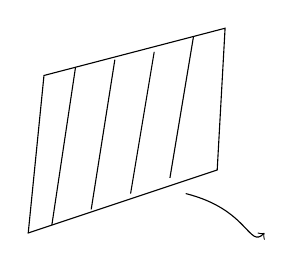
\begin{tikzpicture}[x=1cm,y=1cm]\draw(0,2)--(2.3,2.6)--(2.2,.8)--(-.2,0)--cycle;\draw(.1,.1)--(.4,2.1);\draw(.6,.3)--(.9,2.2);\draw(1.1,.5)--(1.4,2.3);\draw(1.6,.7)--(1.9,2.5);\draw[->](1.8,.5)..controls(2.6,.3)and(2.6,-.2)..(2.8,0);\end{tikzpicture}}
Plus \uline{gén.}, si $\unsure{\operatorname{Liss}(k_0)|\operatorname{Linc}(k_0)}$ est la catégorie des $k_0$-schémas \uline{augmentés}\inserted{$k_0$-}\unsure{morphismes} \deleted{\unsure{$\xi$}} des \deleted{\unsure{$\xi$}} $\operatorname{Sp}\operatorname{Sym}^*_{\unsure{k_0|k}}(M_0)$, \deleted{\unsure{on}} il y a un foncteur $X\unsure{-|\to}\widehat X^{(\mathcal A_*)}$ de $\unsure{\operatorname{Liss}(k_0)|\operatorname{Linc}(k_0)}$ vers les $\mathcal A_*$-schémas formels, commutant aux produits finis, et transformant objets groupes en objets groupes $\ldots$
\margin{$\mathcal O_{\mathcal A_*}(X)\subset\mathcal O(X)$.\quad
$\operatorname{Hom}_{\mathcal A_*\text{ form.}}\text{ ``}(X,X_1)\text{''}\quad \operatorname{Hom}_{k\text{-formel}}(X,X_1)$}
\margin{Modules \inserted{(lisses de t.f.)} $\mathcal A_*$ formels sur les schémas $\mathcal A_*$-formels$\ldots$\quad
\deleted{\unsure{Le sous}} fibré vectoriel $\mathcal A_*$ formel associé\quad
$\overline{\mathbf V}_{\mathcal A_*}(M)$, -- $W_{\mathcal A_*}(M)$}
\figure{\begin{tikzpicture}[x=1cm,y=1cm]\draw (0,5)--(0,2.5)..controls(.1,2.3)and(.2,2.3)..(.3,2.3)--(.3,.5)..controls(.3,.2)and(0,0)..(-.3,0);\draw[-](0,4.5)--(-.8,4.5);\end{tikzpicture}}
\margin{10}
